\chapter{Objetivos del proyecto, planificación y motivación personal}
\label{chapter:objetivos}
\section{Objetivos del proyecto}

Este proyecto se contextualiza dentro del marco de la metodología de encuestas. En concreto, se centra en las encuestas longitudinales a hogares, y dentro de ese campo pone el foco en la predicción de la participación de los hogares en olas posteriores a su primera colaboración. La encuesta elegida para el proyecto es la Encuesta Financiera de las Familias (EFF), una encuesta de referencia para investigaciones sobre finanzas de los hogares.

El \textbf{objetivo principal} de este proyecto es desarrollar un modelo de predicción basado en métodos de machine learning que ayude a predecir si un hogar que ha participado en al menos una ola de la EFF volverá a hacerlo en olas posteriores.

Para poder desarrollar ese modelo, es necesario completar una serie de \textbf{objetivos secundarios}. Estos objetivos se agruparán en 5 fases:

\begin{enumerate}[noitemsep]
    \item Hacer una revisión del estado del arte sobre el Panel Attrition y las metodologías de Machine Learning aplicadas a su predicción.
    \item Recolección de datos. Preferentemente, obtener un conjunto de datos que contenga:
    \begin{enumerate}
        \item Las respuestas de los hogares al cuestionario de la EFF.
        \item Paradata sobre el proceso de creación de la encuesta.
        \item Características de los entrevistadores.
    \end{enumerate}
    \item Análisis exploratorio de los datos. Identificar patrones dentro de los datos que puedan estar relacionados con el panel attrition.
    \item Preprocesar los datos para entrenar modelos de machine learning.
    \item Modelado y evaluación de modelos de predicción basados en métodos de machine learning.
    \item Interpretación del mejor modelo y redacción de conclusiones.
\end{enumerate}

\section{Planificación del proyecto}

La planificación de este proyecto se va a dividir en 5 fases. La asignación temporal a cada una de ellas se ha realizado de acuerdo a la estructura de contenidos del Plan Docente y al calendario de la asginatura.

\begin{enumerate}[noitemsep]
    \item Fase 1: Contiene la definición del proyecto y la planificación del TFM. Abarca las dos primeras semanas del proyecto, del 27 de septiembre al 10 de octubre.
    \item Fase 2: Contiene las tareas de la revisión de la literatura y la caracterización del panel attrition de la EFF. Abarcará desde el 11 de octubre al 23 de octubre.
    \item Fase 3: Contiene las tareas de recolección de datos, análisis exploratorio de dichos datos, preprocesamiento para entrenar los modelos de machine learning, modelado y evaluación de los modelos de predicción, y la interpretación de los modelos y la redacción de conclusiones. Esta fase es la más duradera y abarcará desde el 17 de octubre al 19 de diciembre.
    \item Fase 4: En esta fase se procederá a la redacción de la memoria del TFM y la preparación de una presentación audiovisual sobre el proyecto. Abarcará desde el 20 de diciembre al 18 de enero.
    \item Fase 5: En esta fase final se procederá a la defensa del TFM. Esa etapa abarcará desde el 22 de enero hasta el 4 de febrero.
\end{enumerate}

 En la figura \ref{fig:gantt} puede observarse la distribución temporal y el tiempo dedicado a cada tarea en un diagrama de Gantt.


\begin{figure}
	\centering
	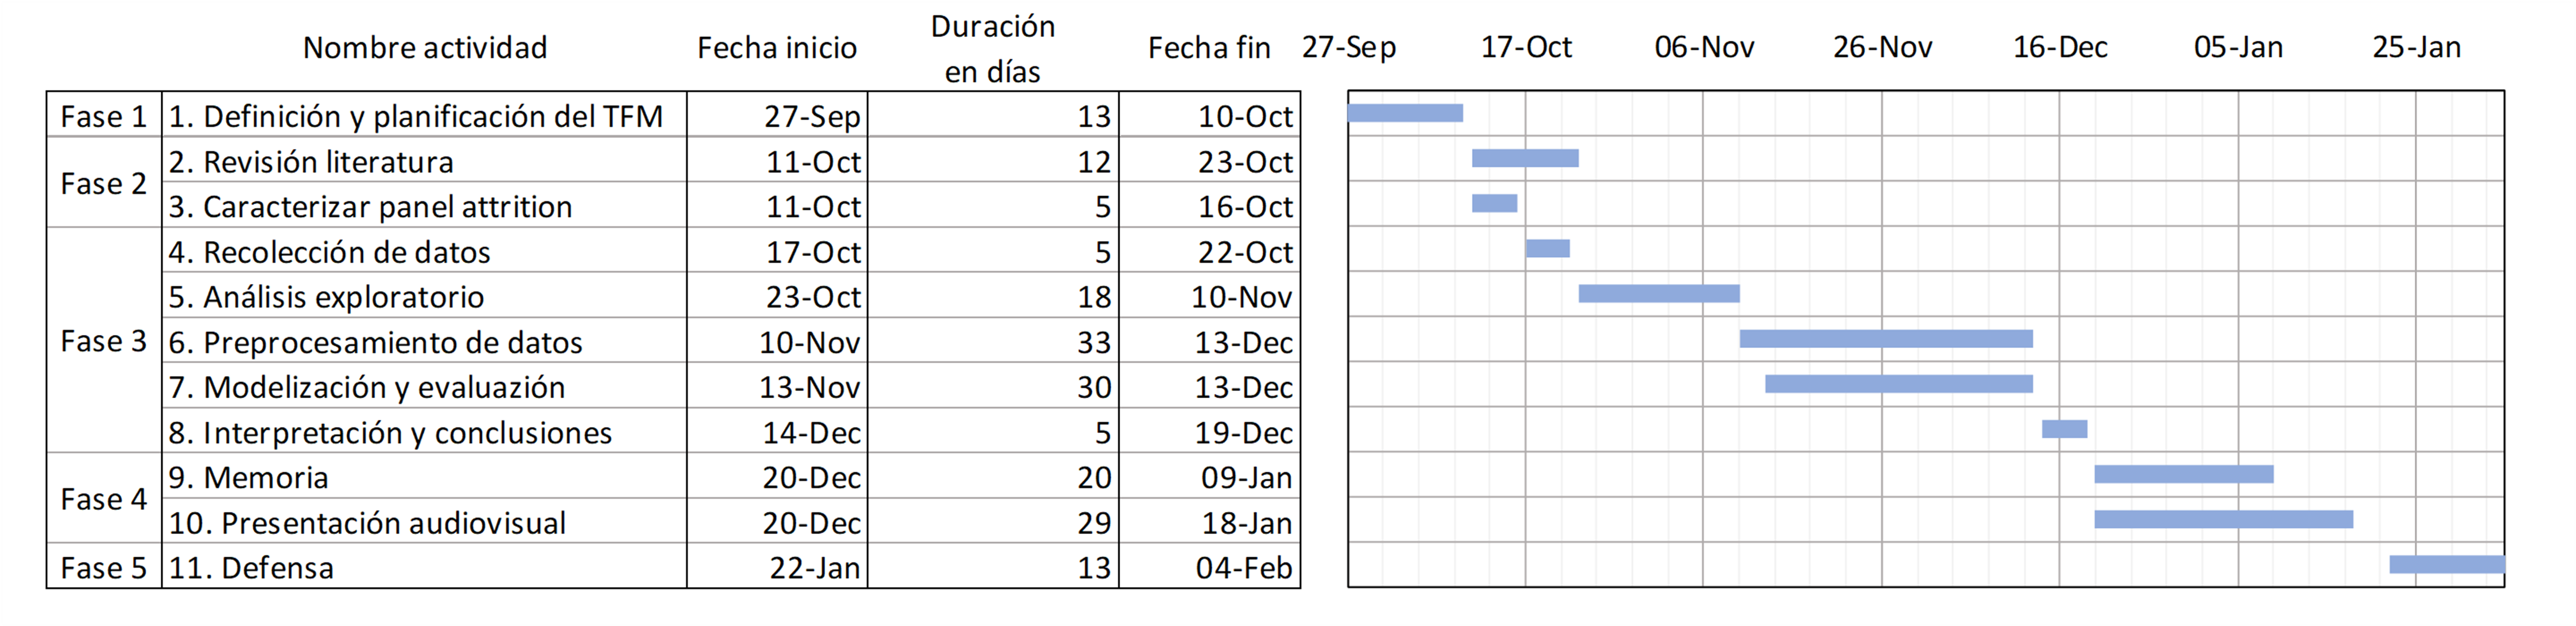
\includegraphics[width=1\textwidth]{figs/Gantt_diagram.png}
	\caption{Planificación de las actividades del TFM}
	\label{fig:gantt}
\end{figure}

\section{Motivación personal}

Trabajo para el Banco de España, y formo parte del equipo que elabora la Encuesta Financiera de las Familias (EFF) desde principios de 2015. He participado en la elaboración de sus cuatro últimas ediciones (EFF2014, EFF2017, EFF2020 y EFF2022) y con los años ha crecido mi interés por la metodología de encuestas y el potencial que tienen para recoger información sobre fenónemos que de otra manera serían difíciles de captar. La EFF es una fuente de información de referencia en el campo de las finanzas de los hogares y eso hace más importante realizar trabajos y esfuerzos para garantizar e incluso mejorar la calidad de sus datos. En ese sentido, la gran cantidad de paradatos que se generan durante cada ola ofrecen muchas oportunidades para aprender sobre todo el proceso y encontrar maneras de mejorarlo.

Por otro lado, en los últimos años ha aumentado cantidad de datos que se generan durante la encuesta y también su variedad, tomando espacecial relevancia los audios de las entrevistas y los comentarios de texto escritos por los entrevistadores, que se han convertido en herramientas fundamentales de los procesos de revisión de calidad de los datos. Los métodos y las herramientas desarrolladas en el campo de la ciencia de datos abren un mundo de posibilidades para poder analizar y explotar toda esa información.

Finalmente, sobre el Panel Attrition, considero que la etapa más importante de la elaboración de la EFF es el trabajo de campo. En ella se contacta a los hogares, se les convence para participar en la encuesta y se realizan las entrevistas. Marca el devenir las siguientes etapas, y también el nivel de calidad de los datos. Por esa razón, es importante conseguir la colaboración de los hogares. Especialmente la de los hogares panel, ya que representan una proporción importante de la muestra, y no convercerles puede llegar a ser muy costoso. Y es un área que en la EFF no se ha podido explorar hasta. Es una gran oportunidad para aprender.